\documentclass[11pt]{article}
\usepackage[margin=1in]{geometry}
\usepackage{amsmath,amssymb,booktabs,graphicx,hyperref}
\usepackage[numbers,sort&compress]{natbib}
\usepackage{lineno}
\usepackage{placeins}
\hypersetup{hidelinks}
\linenumbers
\graphicspath{{figures/}}
\setlength{\emergencystretch}{2em}

\title{Cross-fitted selective recovery under controlled multi-sensor corruption}
\author{Riyang Luo$^{1,*}$\\
\small $^1$School of Mechanical and Power Engineering, Nanjing Tech University,\\
\small 30 South Puzhu Road, Nanjing 211816, Jiangsu Province, China\\
\small $^*$Correspondence: lry@njtech.edu.cn}
\date{}

\begin{document}
\maketitle

\begin{abstract}
An available sensor group can remain in the inference path after its representation has been corrupted. A recovery model may then correct a wrong decision or overturn a correct one. We address this trade-off with paired clean--faulted training and a cross-fitted router that selects between a bounded base model and a recovery-supervised endpoint without test labels or fault-type inputs. The primary objective is hard-decision safety, measured by negative-transfer prevention, recovery retention and net utility; ranking and probability quality are secondary. On 1,436 held-out observations per mechanism with a controlled fault that reached an available group, the two-pass Lite-CF router prevented 94.7\% of recovery-induced negative transfers while retaining 9.7\% of available corrections. Its mean macro-AUROC was 0.8151, compared with 0.8115 for the base model and 0.8175 for unconditional recovery. Router calibration was sparse and model-specific: only 89.7 correctness disagreements informed each fit on average, and repeated thresholds ranged from 0.525 to 0.90. On the present fixed test set, fitted-pair intervals were positive for Gaussian and stuck-at corruption but not uniformly for offset or drift. At equal correction and harm values, Lite-CF gained 15.8 correct decisions per 10,000 strict observations, but complete-stream utility was negative at 0\% and 10\% controlled-fault prevalence. The strict-set advantage disappeared when one harm exceeded approximately 2.9 corrections. Unsupported deployments must retain the base endpoint. The evidence supports a conservative risk-control layer for controlled available-group corruption, not general predictive superiority, natural-failure recovery or device-independent field performance.
\end{abstract}

\noindent\textbf{Keywords:} multi-sensor fusion; sensor corruption; fault-tolerant classification; selective recovery; negative transfer; cross-fitting

\section{Introduction}

Scientific and industrial systems increasingly combine several channels whose availability and fidelity can change after deployment. Missing inputs, delayed diagnostics and distribution shifts can invalidate a model even when its architecture performs well on a static benchmark \citep{liu2025deployment,chakraborti2025personalized,mitra2023structured,wu2026survey}. This problem is distinct from ordinary random missingness because a faulty sensor can remain present and produce plausible but biased, clipped, noisy or unresponsive measurements. A robust fusion rule must therefore decide not only whether a channel exists, but how strongly it should influence the prediction.

Several training strategies improve tolerance to absent or inconsistent sources. Modality dropout, masking and self-distillation expose models to missing inputs \citep{neverova2016moddrop,li2024umdf,woo2023practices}. Representation refinement, gradient decoupling and expert routing address source imbalance or train--test mismatch \citep{wang2024gradient,mckinzie2023mismatch,yao2024drfuse,huang2025mgr}. Reliability-aware fusion additionally uses predictive uncertainty, learned credibility or rejection \citep{gao2024aleatoric,cho2025cocoon,park2025mome,sidheekh2025credibility,liu2025rejection,rabanser2025selective}. Quality-aware multimodal fusion (QMF) provides a published failure-aware comparator by deriving modality confidence from predictive energy and aligning confidence with historical loss trajectories \citep{zhang2023qmf}. These approaches establish useful design patterns, but they do not make an arbitrary weighting response physically calibrated or comparable across sensors.

Sensor-fault diagnosis has a complementary engineering literature. Redundant sensor networks can localize offset, drift, noise, peaks and stuck responses, and can distinguish local sensor faults from global system changes \citep{kullaa2011distinguishing,kullaa2013sensor,helwig2015sensorfault}. Hydraulic condition-monitoring studies further show the value of heterogeneous pressure, flow, temperature, power and vibration measurements for component-state classification \citep{helwig2015condition,ma2021multirate,keleko2023hydraulic,yildirim2025hydraulic}. These studies motivate physically defined sensor groups and independent condition-monitoring validation rather than arbitrary computational groupings alone.

Most open benchmarks nevertheless encode sensor failure through simulation, laboratory intervention or post hoc feature corruption. A recent public AHU resource instead provides one year of building-management-system records from an office, an auditorium and a hospital, with return- and supply-air temperature sensor faults annotated by experienced HVAC engineers \citep{wang2025ahuoperational,wang2024ahudataset}. These labels create a useful external field test, although they are rule- and expert-adjudicated operational annotations rather than maintenance-confirmed hardware replacement events.

Recent AHU studies show that the direct diagnosis problem differs from fault-tolerant recovery. Transformer models can exploit long temporal dependencies within a continuously operating hospital, while attention-based transfer and temporal--contextual learning explicitly address building shift and limited labels \citep{wang2025ahutransformer,feng2024attention,wang2026temporal}. These architectures preserve fault signatures to identify the failure itself. In contrast, fault-tolerant classification seeks to suppress corrupted evidence while retaining another target, so superiority in one task need not transfer to the other.

We study paired-degradation responsive fusion (PDRF). ``Responsive'' denotes an operational change in fusion weight after a controlled sensor degradation; it does not imply physical health, calibrated risk or sensor variance. Each training observation is paired with a view in which one available sensor group is degraded. The model learns a bounded response, and directional losses encourage the affected sensor's response to rise and its fusion weight to fall. The formulation does not invoke an identifiable causal counterfactual. Predictive calibration is evaluated separately because discrimination, uncertainty and calibration are different properties \citep{kendall2017uncertainties,hullermeier2021uncertainty,lakshminarayanan2017ensembles,guo2017calibration,ovadia2019trust,minderer2021calibration,vaicenavicius2019calibration}.

The study makes four contributions. First, it defines a strict recovery estimand that includes only controlled interventions that reach an available sensor group. Second, it formulates selective recovery as hard-decision risk control and cross-fits both the routing score and operating threshold. The primary Lite-CF implementation uses six endpoint features and two forward passes. Third, it audits the sparse routing problem through repeated grouped splits, coefficient and sign stability, regularization paths, calibration-size sensitivity, an all-row three-outcome model, a shallow tree and a staged cascade. Fourth, it separates mechanism-fixed, batch-fixed and fitting-seed variation and reports the final routed probabilities on discrimination and calibration metrics. The title and claims are limited to controlled corruption. Hydraulic results are single-rig sensitivity evidence, and expert-annotated air-handling-unit diagnosis remains a negative task boundary because it lacks an independent downstream recovery target.

\section{Related work}

\subsection{Missing and unreliable sensor inputs}

Missing-data mechanisms affect the interpretation of any robustness experiment \citep{little2019missing}. Random sensor dropout tests tolerance to absent channels, whereas the present study targets channels that remain available but become corrupted. Corruption augmentation and consistency distillation can improve this setting, but they can also make an apparently novel fusion rule indistinguishable from robust training. Our comparator design therefore gives the main gates identical paired degradations, labels, minibatches and additional forward passes, and separately evaluates early and uniform fusion with clean distillation and modality-dropout self-distillation.

\subsection{Bounded operational responses and probability calibration}

Input-dependent losses can represent aleatoric variation under valid probabilistic assumptions, whereas PDRF uses its bounded response only for weighting \citep{kendall2017uncertainties,hullermeier2021uncertainty}. Response ordering and isotonic audits therefore do not convert it into physical variance. Probability quality is assessed separately with NLL, Brier score, multiple ECE definitions and temperature scaling because calibration depends on both multiclass structure and binning \citep{vaicenavicius2019calibration,kull2019dirichlet,mortier2023classifier}. Entropy weighting, deep ensembles and conformal sets provide uncertainty-oriented comparators, not device-health estimates \citep{lakshminarayanan2017ensembles,podkopaev2021distribution}. Cross-building AHU controls likewise distinguish source-only GroupDRO from target-feature adaptation by CORAL or target normalization \citep{sun2016coral,sagawa2020groupdro,mirza2022normalization}.

\subsection{Selective prediction and model fallback}

Selective classification and reject-option learning trade coverage for lower predictive risk \citep{elyaniv2010selective,geifman2019selectivenet,franc2023reject}; recent work additionally studies selection under distribution shift \citep{liang2024selective}. Learning-to-defer methods route difficult cases to a human or another expert whose error pattern may differ from that of the primary predictor \citep{mozannar2020defer,tailor2024population}. Classifier cascades explicitly trade predictive accuracy against evaluation cost, while dynamic classifier and ensemble selection estimate which member is locally competent \citep{chen2012cascade,cruz2018dynamic}. Mixture-of-experts routing provides a related differentiable allocation mechanism \citep{park2025mome}. The present fallback problem is narrower: both endpoints are fixed models of the same sensor-fusion task, no observation is rejected, and the selector specifically controls recovery-induced negative transfer while retaining corrections. Its operating curve is therefore prevention versus retained recovery, rather than conventional risk versus coverage, human deferral utility or average cascade cost.

\subsection{Evidence and statistical estimands}

Classifier comparisons can change with the resampling unit and evaluation estimand \citep{dietterich1998tests,demsar2006statistical}. Optimization seeds describe repeated fitting, whereas sample bootstrap intervals describe a fixed set of fitted predictors \citep{efron1994bootstrap}. McNemar's paired test evaluates discordant hard decisions on the same observations \citep{mcnemar1947correlated}. We report these levels separately and do not treat observations from one instrument as independent devices. Precision--recall metrics are included because class imbalance can make ROC summaries incomplete \citep{saito2015precision}.

\section{Methods}

\subsection{Problem definition}

For observation $i$ and sensor group $m$, let $\mathbf{x}_{im}\in\mathbb{R}^{d}$ be the feature vector, $a_{im}\in\{0,1\}$ the availability indicator, $q_{im}\in(0,1]$ an optional diagnostic-quality covariate and $y_i\in\{1,\ldots,C\}$ the target. PDRF estimates
\begin{equation}
p\!\left(y_i\mid\{\mathbf{x}_{im},a_{im},q_{im}\}_{m=1}^{M}\right).
\end{equation}
When no quality metadata are available, all $q_{im}$ equal one. Every evaluated observation contains at least one available group. If all groups are unavailable, the implementation abstains before inference because normalized fusion is undefined.

For the routing audit, let $b_i$ indicate that the base endpoint is correct, $r_i$ that the recovery endpoint is correct and $s_i$ that the router emits the recovery output. Table~\ref{tab:event-notation} fixes the event terminology used throughout.

\begin{table}[ht]
\centering
\caption{Hard-decision event definitions and denominators. $N_C$ and $N_H$ count correction and harm opportunities; $n_C$ and $n_H$ count retained corrections and realized harms. Prevention is $1-n_H/N_H$, whereas recovery retention is $n_C/N_C$.}
\label{tab:event-notation}
\resizebox{\textwidth}{!}{\begin{tabular}{lll}
\toprule
Quantity & Event definition & Reported rate \\
\midrule
Correction & $\neg b_i\wedge r_i$ & retained corrections / corrections \\
Negative transfer & $b_i\wedge\neg r_i$ & prevented harms / harm opportunities \\
Residual harm & $b_i\wedge\neg r_i\wedge s_i$ & residual harms / observations \\
Recovery selection & $s_i$ & selected recovery outputs / observations \\
Harmful switch & $b_i\wedge\neg r_i\wedge s_i$ & harmful switches / observations \\
Net correct change & corrections retained $-$ harms realized & events per 10,000 \\
\bottomrule
\end{tabular}
}
\end{table}

\subsection{Architecture and bounded weighting}

Each sensor group is encoded by affine layers $d\rightarrow64\rightarrow32$, with a ReLU after each hidden affine transformation and no normalization or dropout. A biased linear $32\rightarrow C$ output produces group-specific logits $\boldsymbol{\mu}_{im}$. The response head is exactly $\operatorname{Linear}(32,16,\mathrm{bias}=\mathrm{true})$, ReLU, then $\operatorname{Linear}(16,1,\mathrm{bias}=\mathrm{true})$. There is no activation after the final linear layer, so its raw response $u_{im}$ can be positive or negative. The bounded operational response is
\begin{equation}
\begin{aligned}
r_{im}&=B\tanh(u_{im}/B),\\
-B&<r_{im}<B.
\end{aligned}
\label{eq:score}
\end{equation}
where the prespecified main setting uses $B=3$. This layer placement matches the released implementation and gives the symmetric open interval in Eq.~\eqref{eq:score}. Across 17,650 clean and faulted seed--observation responses from 10 fitted RO-PDRF-Full models, the observed float32 range was $-2.899454$ to $3.000000$; the latter is numerical rounding of a value below the mathematical open boundary. Clean responses ranged from $-2.757962$ to $2.997449$. Unnormalized and normalized weights are
\begin{equation}
\begin{aligned}
\widetilde w_{im}&=a_{im}q_{im}\exp(-\beta r_{im}),\\
 w_{im}&=\frac{\widetilde w_{im}}{\sum_k\widetilde w_{ik}}.
\end{aligned}
\label{eq:weights}
\end{equation}
with $\beta=0.25$. Fused logits are $\boldsymbol{\ell}_i=\sum_mw_{im}\boldsymbol{\mu}_{im}$. The implementation applies a $10^{-6}$ lower guard to the normalization denominator, but the guard is inactive under the stated input constraints because every observation has at least one available group and $q_{im}\geq0.01$ after clipping.

This construction differs from an unconstrained softmax gate in three testable ways. First, the weight is factorized into availability, an optional externally measured quality term and one bounded operational response; it is not an unrestricted function of the concatenated sensor representation. Second, the perturbed group is known during paired degradation, so its response and normalized weight receive directional supervision rather than only a task-gradient signal. Third, the same response that controls fusion is regularized by a group-specific predictive loss. Thus the response is operationally coupled to group evidence, although it is not asserted to be a physical health variable.

The factorization also gives two elementary stability properties. For an available group, fixed $q$ and any $k\ne m$,
\begin{equation}
\begin{aligned}
\frac{\partial w_{im}}{\partial r_{im}}&=-\beta w_{im}(1-w_{im})\leq0,\\
\frac{\partial w_{ik}}{\partial r_{im}}&=\beta w_{ik}w_{im}\geq0.
\end{aligned}
\label{eq:monotone}
\end{equation}
For two available groups with equal quality, bounded responses imply
\begin{equation}
e^{-2\beta B}<\frac{\widetilde w_{im}}{\widetilde w_{ik}}<e^{2\beta B}.
\label{eq:ratio}
\end{equation}
At $B=3$ and $\beta=0.25$, one response alone can therefore create at most a 4.48-fold unnormalized-weight ratio between equal-quality groups. These properties do not guarantee that the learned ordering is correct; the experiments separately test that question.

The response regularizer, retained as $\mathcal L_{\mathrm{score}}$ in the implementation for reproducibility, combines a bounded heteroscedastic-style term and a boundary penalty. For a minibatch $\mathcal B$, write $s_{im}=\omega_{y_i}[-\log\operatorname{softmax}(\boldsymbol{\mu}_{im})_{y_i}]$, where $\omega_c=n/(Cn_c)$ is the training-set class weight, and let $h_{im}=e^{-r_{im}}s_{im}+r_{im}$. Then
\begin{equation}
\mathcal L_{\mathrm{score}}=
\frac{\sum_{i\in\mathcal B}\sum_m a_{im}h_{im}}
{\sum_{i\in\mathcal B}\sum_m a_{im}},
\end{equation}
\begin{equation}
\mathcal L_{\mathrm{bound}}=
\frac{\sum_{i\in\mathcal B}\sum_m a_{im}(r_{im}/B)^4}
{\sum_{i\in\mathcal B}\sum_m a_{im}}.
\end{equation}
Because cross-entropy is non-negative and $r_{im}>-B$, $\mathcal L_{\mathrm{score}}>-B$. The complete objective therefore has a finite lower bound. This statement concerns optimization stability, not calibration of the bounded operational response.

\subsection{Paired degradation and directional losses}

For each minibatch observation, one available group $m^*$ is drawn from a fixed training prior. A retention factor $\rho_i\sim\operatorname{Uniform}(0.15,0.50)$ controls additive Gaussian degradation with scale $2.5(1-\rho_i)$. In half of the pairs, $q_{im^*}$ is multiplied by $\rho_i$; otherwise it is unchanged. Let primed symbols denote the degraded view and $d_i=1-\rho_i$.

The clean and degraded task losses use the class-weighted mean implemented by PyTorch. With $e_i(\boldsymbol\ell)=-\log\operatorname{softmax}(\boldsymbol\ell)_{y_i}$,
\begin{equation}
\begin{aligned}
\mathcal L_{\mathrm{task}}&=
\frac{\sum_{i\in\mathcal B}\omega_{y_i}e_i(\boldsymbol\ell_i)}
{\sum_{i\in\mathcal B}\omega_{y_i}},\\
\mathcal L_{\mathrm{deg}}&=
\frac{\sum_{i\in\mathcal B}\omega_{y_i}e_i(\boldsymbol\ell'_i)}
{\sum_{i\in\mathcal B}\omega_{y_i}}.
\end{aligned}
\label{eq:task-losses}
\end{equation}
Let $\mathcal V_{\mathcal B}=\{i\in\mathcal B:\sum_m a_{im}>1\}$ denote observations for which the selected group can be removed while another group remains. For $i\in\mathcal V_{\mathcal B}$, the removal prediction $\mathbf p_i^{(-m^*)}$ defines a severity-interpolated target $\mathbf t_i$; write $\widehat{\mathbf t}_i=\operatorname{stopgrad}(\mathbf t_i)$:
\begin{equation}
\begin{aligned}
\mathbf t_i&=(1-d_i)\mathbf p_i+d_i\mathbf p_i^{(-m^*)},\\
\mathcal L_{\mathrm{cons}}&=\frac{1}{|\mathcal V_{\mathcal B}|}
\sum_{i\in\mathcal V_{\mathcal B}}
\|\mathbf p'_i-\widehat{\mathbf t}_i\|_2^2.
\end{aligned}
\end{equation}
If $\mathcal V_{\mathcal B}$ is empty, $\mathcal L_{\mathrm{cons}}$ and the removal-dependent directional terms are omitted, equivalently set to zero. Directional terms operate on the affected normalized weight and raw response and are averaged over eligible observations. With $[z]_+=\max(0,z)$ and $\Delta w_i=w'_{im^*}-w_{im^*}$,
\begin{equation}
\mathcal L_{\mathrm{mono}}=|\mathcal V_{\mathcal B}|^{-1}
\sum_{i\in\mathcal V_{\mathcal B}}[\Delta w_i]_+.
\end{equation}
With $\gamma_i=0.5d_i/0.85$ and $\Delta r_i=\operatorname{stopgrad}(r_{im^*})-r'_{im^*}$, the response-ranking term is
\begin{equation}
\mathcal L_{\mathrm{rank}}=|\mathcal V_{\mathcal B}|^{-1}
\sum_{i\in\mathcal V_{\mathcal B}}[\gamma_i+\Delta r_i]_+.
\end{equation}
The final loss is
\begin{equation}
\begin{aligned}
\mathcal L={}&\mathcal L_{\mathrm{task}}+0.20\mathcal L_{\mathrm{score}}\\
&+0.50\mathcal L_{\mathrm{bound}}+0.15\mathcal L_{\mathrm{deg}}\\
&+0.10\mathcal L_{\mathrm{cons}}+0.05\mathcal L_{\mathrm{mono}}\\
&+0.15\mathcal L_{\mathrm{rank}}.
\end{aligned}
\label{eq:objective}
\end{equation}

\begin{figure}[ht]
\centering
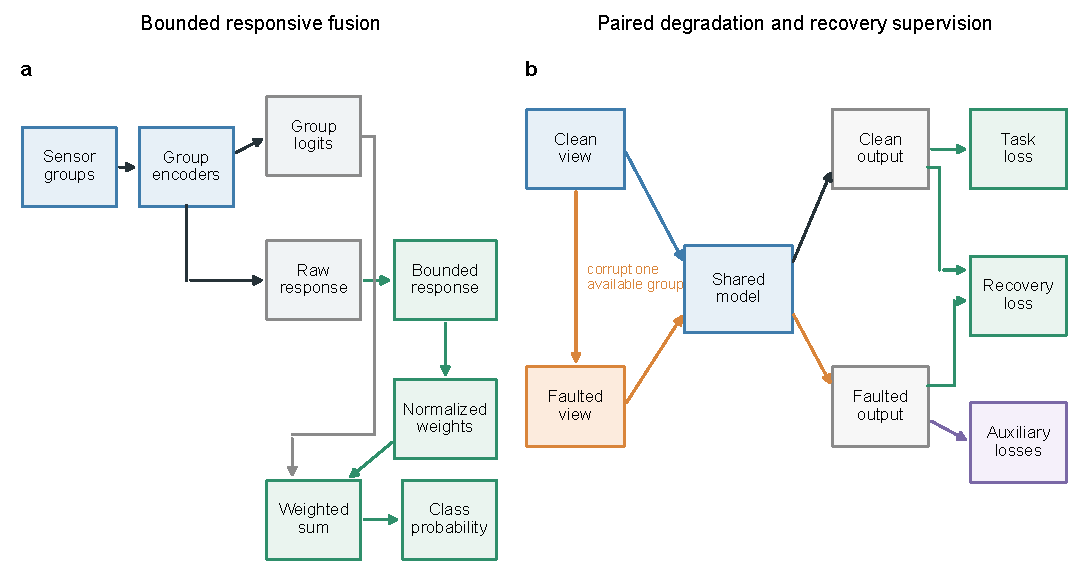
\includegraphics[width=\textwidth]{figure1_method_framework.pdf}
\caption{\textbf{Bounded responsive fusion and recovery supervision.} \textbf{a}, Each sensor group produces class logits and a bounded operational response. Availability, optional diagnostic quality and the response determine normalized fusion weights. Distinct connector ports separate the logit and weight contributions to the fused prediction. \textbf{b}, Clean and faulted views share model parameters. The detached clean prediction supervises recovery of the faulted prediction; proper-scoring and ranking terms are auxiliary controls.}
\label{fig:method}
\end{figure}
\FloatBarrier

\subsection{Comparators and mechanism ablations}

Early fusion concatenates zero-filled group features, masks and quality values before a $128\rightarrow64\rightarrow C$ multilayer perceptron; uniform fusion averages group logits. Both receive the same paired degradation and degraded-task loss as PDRF. CAGF concatenates four 32-dimensional group representations, masks and quality values before an unrestricted $64\rightarrow M$ softmax gate. It shares PDRF's paired-degradation, consistency and normalized-weight monotonicity losses. Direct weight ranking adds a gate-weight margin, while the quality-only control uses $a_{im}q_{im}$ without a learned response.

RO-AT-GATE tests stronger cross-group interaction. It adds learned group identities to 32-dimensional tokens and applies one four-head attention layer with a 64-unit feed-forward block; unavailable groups are masked. A shared $32+2\rightarrow16\rightarrow1$ head maps each contextualized token, availability and quality to an unrestricted softmax gate. The 26,809-parameter model receives the same paired views and recovery objective as RO-CAGF. It is a sensor-group attention control, not a reproduction of a task-specific vision or language system \citep{li2024umdf,gao2024aleatoric,cho2025cocoon}.

RO-MER supplies a sample-dependent multi-expert control motivated by failure-resilient routing \citep{park2025mome}. It combines one classifier per physical group with a joint 64-unit expert and a separate 64-unit router. The prediction uses the resulting $(M+1)$-expert distribution. Losses requiring physical-group weights use the differentiable allocation
\begin{equation}
w^{\mathrm{eff}}_{im}=\alpha_{im}+\alpha_{iJ}\frac{a_{im}}{\sum_k a_{ik}}.
\label{eq:mer-effective}
\end{equation}
The joint probability is distributed uniformly only for shared monotonicity and gate regularization; Eq.~\eqref{eq:mer-effective} does not alter the prediction. RO-MER has 35,811 parameters and uses the same faults, batches, seeds and checkpoint rule as RO-CAGF and RO-PDRF-Full.

The complete RO-MER objective is
\begin{equation}
\begin{aligned}
\mathcal L_{\mathrm{RO\text{-}MER}}={}&\mathcal L_{\mathrm{task}}+0.15\mathcal L_{\mathrm{deg}}+0.10\mathcal L_{\mathrm{cons}}+0.05\mathcal L_{\mathrm{mono}}\\
&+0.30\mathcal L_{\mathrm{rec}}+0.05\mathcal L_{\mathrm{Brier}}+0.10\mathcal L_{\mathrm{AUC}}+0.005\mathcal L_{\mathrm{router}},
\end{aligned}
\label{eq:mer-objective}
\end{equation}
Here $\mathcal L_{\mathrm{router}}$ is the clean-plus-degraded Kullback--Leibler divergence from $\mathbf w_i^{\mathrm{eff}}$ to uniform allocation over available groups. RO-CAGF uses the same coefficients with native softmax weights; RO-PDRF-Full substitutes its response-interior penalty. Recovery supervision, proper scoring, pairwise ranking, paired views and task losses are otherwise matched.

We additionally adapt Quality-aware Multimodal Fusion (QMF) to the same four sensor groups while retaining its detached energy-confidence fusion and historical-loss ranking rule \citep{zhang2023qmf}. This QMF-PD control shares the present encoders, corruptions, optimizer, split and checkpoint criterion; it is a sensor-group adaptation rather than an exact reproduction of the original backbones or tasks. Implementation choices and sensitivity variants are specified in the Supplementary Information.

PDRF contains 19,740 trainable parameters on the chemical array, compared with 26,588 for CAGF and DWR, 35,811 for RO-MER, 26,182 for early fusion and 17,560 for uniform fusion. Ablations comprise paired degradation only (PD-ONLY), paired degradation plus normalized-weight monotonicity (PD-MONO), paired degradation plus response ranking (PD-RANK), the complete objective without $\mathcal L_{\mathrm{score}}$ (NO-LSCORE), and $\mathcal L_{\mathrm{score}}$ without $\mathcal L_{\mathrm{rank}}$ (LSCORE-NO-LRANK). A PDRF-NOQ model is trained and tested with all quality values fixed to one.

\subsection{Recovery-oriented extension}

Reducing an affected group's weight did not ensure prediction recovery. RO-PDRF therefore retains the PDRF architecture and distils the degraded prediction from the detached clean-view prediction. Writing $\widehat{\mathbf p}_i=\operatorname{stopgrad}(\mathbf p_i)$ gives
\begin{equation}
\mathcal L_{\mathrm{rec}}=\frac{1}{|\mathcal V_{\mathcal B}|}
\sum_{i\in\mathcal V_{\mathcal B}}D_{\mathrm{KL}}\!\left[\widehat{\mathbf p}_i\,\|\,\mathbf p'_i\right].
\end{equation}
$\mathcal L_{\mathrm{rec}}$ requires at least two available groups and is omitted when $\mathcal V_{\mathcal B}$ is empty. This excluded $0.386\%\pm0.052\%$ of 5,933 training rows across seeds. PDRF plus $0.30\mathcal L_{\mathrm{rec}}$ defines RO-PDRF-Lite. Label-assisted, confidence-weighted, exponential-moving-average and agreement-gated teachers remain supplementary controls; the deployed selector uses no held-out label \citep{tarvainen2017mean}.

Second, multiclass Brier losses on clean and degraded predictions provide proper-scoring supervision,
\begin{equation}
\begin{aligned}
\mathcal L_{\mathrm{Brier}}={}&\frac{1}{|\mathcal B|}\sum_{i\in\mathcal B}\|\mathbf p_i-\mathbf e_{y_i}\|_2^2\\
&+\frac{1}{|\mathcal B|}\sum_{i\in\mathcal B}\|\mathbf p'_i-\mathbf e_{y_i}\|_2^2.
\end{aligned}
\end{equation}
The Brier term is unweighted; class weights remain confined to cross-entropy. A weak log barrier then discourages boundary occupancy without removing the quartic penalty. With $\epsilon=10^{-4}$, define $b_\epsilon(r)=-\log\{\max[\epsilon,1-(r/B)^2]\}$, $\bar b_{im}=b_\epsilon(r_{im})+b_\epsilon(r'_{im})$ and $Z_{\mathcal B}=\sum_{i\in\mathcal B}\sum_m a_{im}$:
\begin{equation}
\mathcal L_{\mathrm{interior}}=Z_{\mathcal B}^{-1}
\sum_{i\in\mathcal B}\sum_m a_{im}\bar b_{im}.
\label{eq:interior}
\end{equation}
Unavailable groups are excluded by $a_{im}$; the clamp is numerical. Finally, a smooth one-versus-rest pairwise loss supervises degraded-view class ordering. Let $P_c$ and $N_c$ denote positive and negative minibatch observations, $\mathcal C_{\mathcal B}=\{c:|P_c|>0,|N_c|>0\}$ and $\phi_{ijc}=\operatorname{softplus}[-(\ell'_{ic}-\ell'_{jc})]$:
\begin{equation}
\begin{aligned}
\mathcal L_{\mathrm{AUC}}&=\frac{1}{|\mathcal C_{\mathcal B}|}\sum_{c\in\mathcal C_{\mathcal B}}A_c,\\
A_c&=\frac{\sum_{i\in P_c}\sum_{j\in N_c}\phi_{ijc}}{|P_c||N_c|}.
\end{aligned}
\label{eq:auc}
\end{equation}
The pairwise term is omitted when no class has both outcomes \citep{yang2021pairwise}. RO-PDRF-Full adds $0.30\mathcal L_{\mathrm{rec}}+0.05\mathcal L_{\mathrm{Brier}}+0.005\mathcal L_{\mathrm{interior}}+0.10\mathcal L_{\mathrm{AUC}}$ to Eq.~\eqref{eq:objective}. RO-PDRF-Lite is the practical default, Full is the mechanistic architecture comparator and RO-PDRF-EMA is a Full-based calibration sensitivity. No test observation fits a model or ensemble parameter.

To separate recovery supervision from architecture, we also train recovery-oriented CAGF (RO-CAGF). It receives the same clean-view distillation, Brier and degraded-view ranking losses as RO-PDRF-Full. Its unrestricted softmax gate uses a weak KL-to-uniform regularizer (weight 0.005), whereas RO-PDRF-Full uses the response-interior penalty. The matched data, fixed faults, seeds, minibatches and checkpoint rules isolate architecture subject to this necessary regularizer difference. Regularizer grids, early/uniform-fusion controls, modality-dropout self-distillation and confidence-thresholded distillation are reported in the Supplementary Information \citep{neverova2016moddrop,li2024umdf}.

\subsection{Cross-fitted selective recovery}

Unconditional recovery can repair a wrong base prediction but can also overturn a correct one. We therefore treat routing as hard-decision risk control. Here ``Lite'' means that the router selects between PDRF and the RO-PDRF-Lite recovery endpoint; it does not merely denote a smaller selector. Both endpoints require one ordinary forward pass and have the same 19,740-parameter architecture. The heavier PDRF/RO-PDRF-Full pair is retained only as a supplementary mechanistic and legacy-routing sensitivity.

Batch~7 is divided chronologically into two disjoint halves. The first half fits one scalar temperature per endpoint by minimizing multiclass negative log-likelihood. The second contains two calibration-only realizations of each fault mechanism; only interventions that reach an available affected group enter selector development. Routing features use the temperature-scaled endpoint probabilities. The selected endpoint vector is emitted without probability mixing or post-routing recalibration.

Lite-CF uses six prespecified inputs: base confidence, recovery confidence, their difference, base normalized entropy, recovery normalized entropy and their difference. It receives neither the class label nor fault type at inference. Let $z_{ij}$ denote standardized feature $j$. Feature means and standard deviations are fitted only on the informative training rows inside each cross-fitting fold, then refitted on all informative calibration rows for the final model. An $L_2$-regularized logistic model produces the \emph{conditional preference score}
\begin{equation}
\pi_i=\sigma\!\left(\gamma_0+\sum_{j=1}^{6}\gamma_j z_{ij}\right),
\end{equation}
using calibration rows on which PDRF and RO-PDRF-Lite differ in correctness. The target equals one when recovery is correct and the base endpoint is wrong. This conditional score is not a calibrated reliability probability for the full stream. Lite-CF uses $C=0.05$, the \texttt{lbfgs} solver, balanced class weights, tolerance $10^{-4}$, 2,000 maximum iterations and random state 0.

Coefficient fitting is separated from threshold selection by five-fold stratified group cross-fitting. Realizations and mechanisms from the same calibration observation remain in one fold. Candidate thresholds $0.50,0.525,\ldots,0.90$ are evaluated only on pooled out-of-fold scores. Selection minimizes realized harms, then maximizes selected accuracy and retained corrections; remaining ties use the highest threshold. The formal fits had a mean of 1.5 tied thresholds (range 1--4). Final coefficients are refitted on all informative rows while the threshold remains frozen.

For prospective deployment, mathematical fit is necessary but insufficient. We define an operational support gate requiring at least 25 events in each preference class, median out-of-fold AUROC at least 0.65 across 10 repeated grouped splits, no repeated AUROC below 0.60 and a threshold range no wider than 0.10. Both preference classes must also occur in every fitting fold. This reviewer-requested gate was specified after the frozen experiment and is not used to replace its headline result. A new site that fails any condition must emit PDRF while collecting additional calibration data. The released routing API returns probabilities by default and can optionally return the selected endpoint identity and conditional preference score; routed confidence remains endpoint-specific rather than globally calibrated.

We probe the selected-sample and sparse-event risks in four ways. First, ten repeated grouped splits are run for each of 10 fitted endpoint pairs. Second, standardized coefficient distributions, sign frequencies and $C\in\{0.01,0.05,0.1,0.5,1,5\}$ are audited. Third, calibration groups are subsampled to 25\%, 50\%, 75\% and 100\%. Fourth, an all-row multinomial model predicts three outcomes---base better, equivalent or recovery better---from the same six features. A depth-two tree with minimum leaf size 35 supplies a nonlinear, compute-matched learned baseline. These models use the same grouped cross-fitting and calibration budget as Lite-CF.

Legacy Safe-CF-12, staged-cascade, scalar-rule, random-selection and correctness-opportunity controls are defined and evaluated in the Supplementary Information. They are not part of the primary two-pass deployment chain.

The deployment audit reuses the same endpoints, temperatures, selector and test realization for every stream. It includes the strict fault-applied-and-available subset, a complete 40\%-prevalence mixed stream and a no-imposed-fault stream with the same fixed 20\% group-missingness process. Probability quality is reported separately for endpoint-class agreement and disagreement. The primary outcomes are negative-transfer prevention, recovery retention and
\begin{equation}
U=V_C n_C-C_H n_H-\lambda(P-1),
\label{eq:utility}
\end{equation}
where $n_C$ and $n_H$ are retained corrections and realized harms per 10,000 observations, $V_C$ is correction value, $C_H$ is harm cost, $P$ is mean forward-pass count and $\lambda$ is a pass-cost proxy in correction-equivalents per 10,000 observations. We vary $C_H/V_C$ over 1, 2, 5 and 10, imposed-fault prevalence and $\lambda$. Energy was not measured; forward passes and counted linear-layer FLOPs remain computational proxies.

\subsection{Chemical-sensor dataset and fixed faults}

The UCI Gas Sensor Array Drift Dataset contains 13,910 observations from 16 metal-oxide sensors, six gas classes and 10 acquisition batches over 36 months \citep{vergara2012dataset,vergara2012drift}. Each sensor contributes eight extracted response features. The principal grouping uses four consecutive sensors per group. All models receive the same grouping. Sensitivity analyses additionally use interleaved and five fixed random partitions; no partition is called a physical modality.

Batches 1--6 train the models. Their feature means and standard deviations are the only quantities used for standardization. The same transform is applied to batches 7--10, after which each feature is clipped to $[-8,8]$ before sensor grouping. Thus every reported ``training range'' is the empirical minimum--maximum after training-only standardization and clipping; it is not a physical sensor limit. The first 60\% of Batch~7 selects checkpoints, and the remaining 40\% is reserved for calibration; the routing experiment further divides that calibration partition into temperature and selector halves. Batches 8--10 are never used to fit preprocessing, endpoints, temperatures, selectors or thresholds.

Controlled faults are imposed after this training-only preprocessing in grouped standardized space. The formal test assigns 40\% of observations a scale-3 intervention on group~1 and fixes $q=1$. Fault assignment and 20\% group missingness are generated independently to isolate their factorial effects. This is a stress design, not a claim that all missingness--corruption combinations occur naturally. Of 4,364 test observations, 1,765 are assigned the intervention; group~1 remains available and receives it in 1,436, whereas it is masked in 329. The strict recovery estimand is the former \emph{fault-applied-and-available} subset. Fault indices, missingness masks and intervention values are fixed across methods and optimization seeds.

The complete test set contains 294, 470 and 3,600 observations in batches 8, 9 and 10. Its six class counts are 691, 685, 740, 708, 821 and 719. The corresponding strict-subset batch counts are 91, 165 and 1,180, and its Gaussian class counts are 230, 220, 230, 253, 266 and 237. Complete mechanism-by-batch class tables are supplied in the Supplementary Information.

Checkpoint selection and temperature calibration use separate fault-free views with independently generated 10\% group missingness; no controlled Gaussian, offset, drift or stuck-at intervention is added to either subset. The checkpoint criterion is unweighted cross-entropy on the complete selection subset. For the cross-fitted deployment run, temperature is fitted on the first chronological half of the calibration partition, not an affected subset, by minimizing unweighted multiclass negative log-likelihood. The resulting scalar is specific to each fitted seed and method and is applied unchanged to every deployment stream. Controlled-fault and no-fault deployment streams use the same fixed 20\% group-missingness process so that fault prevalence is the changing factor. Earlier natural-view analyses without imposed test missingness remain supplementary sensitivity evidence.

The expanded fault study crosses four prespecified mechanisms with realizations 70001--70008 and fitted seeds 101--105. Model fitting always uses the Gaussian paired degradation defined above; offset, drift and stuck-at are test-time interventions only. Gaussian faults add independent standardized noise. Offset faults add a featurewise signed displacement. Drift multiplies that displacement by a monotone 0.25--1.00 trajectory over held-out acquisition order. Stuck-at faults replace the affected group's standardized features by a fixed signed vector. Within each realization, all mechanisms share affected rows and missingness masks, while intervention values remain fixed across methods. These are controlled repeats on one instrument.

Table~\ref{tab:fault-plausibility} translates the formal scale into empirical training-distribution displacement. At scale 3, median absolute shifts were 1.89--3.10 training standard deviations and median percentile shifts were 0.36--0.56. Only 9.4--45.7\% of corrupted values remained inside the training 1st--99th percentile interval. The formal setting is therefore a severe standardized stress test, not a typical natural-failure model. Scale-1 and scale-5 summaries and representative inverse-transformed feature examples are reported in the Supplementary Information.

\begin{table}[ht]
\centering
\caption{Fault-plausibility audit in the strict subset. Fractions are calculated featurewise against batches 1--6. ``Training range'' denotes the observed training minimum--maximum, not a physical sensor limit.}
\label{tab:fault-plausibility}
\resizebox{0.94\textwidth}{!}{\begin{tabular}{lrrrr}
\toprule
Mechanism (scale 3) & Median $|\Delta z|$ & Median percentile shift & Within training 1--99\% & Within training range \\
\midrule
Gaussian & 2.015 & 0.360 & 0.379 & 0.609 \\
Offset & 3.000 & 0.538 & 0.332 & 0.632 \\
Drift & 1.888 & 0.440 & 0.457 & 0.697 \\
Stuck-at & 3.105 & 0.557 & 0.094 & 0.656 \\
\bottomrule
\end{tabular}
}
\end{table}

Exploratory controls vary diagnostic-quality metadata, leave-one-group-out training, response bounds, weighting slope, ranking weight, fault group, severity and prevalence. They share observations and fitted models, are not treated as independent replications and do not replace the prespecified main setting. Full specifications and results are reported in the Supplementary Information.

\subsection{Independent hydraulic single-rig sensitivity analysis}

The UCI Condition Monitoring of Hydraulic Systems dataset contains 2,205 raw 60-s cycles from an experimental hydraulic rig and native condition labels for cooler, valve, pump and accumulator states (DOI: \href{https://doi.org/10.24432/C5CW21}{10.24432/C5CW21}) \citep{helwig2018hydraulic,helwig2015condition}. We retain 1,449 cycles marked as stable. Fourteen physical sensors form five groups by measured quantity: six pressure sensors, two flow sensors, four temperature sensors, motor power and vibration. This grouping is defined before model fitting and follows the measurement system rather than a random partition.

Each sensor is summarized by distributional and trend statistics. Unequal group lengths are aligned to 48 inputs; a zero-padded native-order representation audits possible smoothing. The main split preserves acquisition order within every native condition class, assigns contiguous 60\%/15\%/10\%/15\% blocks and removes five cycles at each boundary. A global chronological split would omit some condition classes from training. After guard-band removal, the test counts are 72/72/74 for the three cooler states, 54/54/54/56 for the four valve states, 74/72/72 for the three pump states and 56/54/54/54 for the four accumulator states. Recovery-objective-matched RO-PDRF-Full and RO-CAGF use five matched seeds; controlled pressure- and vibration-group faults affect the same 40\% of test cycles. Component-condition labels are native to the rig, whereas sensor faults remain interventions. Representation and random-split sensitivities are supplementary \citep{ma2021multirate,keleko2023hydraulic,yildirim2025hydraulic}.

\subsection{Real-operational AHU direct-diagnosis boundary analysis}

We additionally use the open real-operational AHU dataset from an auditorium, a hospital and a large office (Figshare DOI: \href{https://doi.org/10.6084/m9.figshare.27147678.v3}{10.6084/m9.figshare.27147678.v3}) \citep{wang2025ahuoperational,wang2024ahudataset}. The binary task uses native, expert-annotated temperature-sensor-fault labels and no artificial test corruption. Seven measurements form five physical groups; each building uses a chronological 60\%/15\%/10\%/15\% split and five matched seeds. The untouched test periods contain 228/9,354 fault records in the auditorium (2.44\%), 1,495/9,362 in the hospital (15.97\%) and 346/19,115 in the office (1.81\%). Return-air/supply-air subtype counts are 179/49, 1,487/8 and 293/53, respectively. Because the label is the sensor fault itself and no independent downstream state is available, this is a negative task-boundary audit, not downstream recovery validation. Detailed shift, adaptation, risk--coverage and conformal analyses are reported in the Supplementary Information \citep{sun2016coral,sagawa2020groupdro,mirza2022normalization,podkopaev2021distribution}.

\subsection{Training, metrics and statistical analysis}

AdamW uses learning rate $2\times10^{-3}$, weight decay $10^{-4}$, batch size 256 and gradient clipping at 5. Chemical-array training uses at most 60 epochs, hydraulic training uses at most 80 and AHU training uses at most 12. Checkpoints minimize unweighted selection cross-entropy and stop after nine epochs without an improvement greater than $10^{-4}$. RO-PDRF-Lite, RO-PDRF-Full, RO-PDRF-EMA and all teacher controls use this identical criterion; no test metric selects a checkpoint or variant. Class weights are $n/(Cn_c)$. No dropout or batch normalization is used.

The primary deployment outcomes are negative-transfer prevention, recovery retention and the utility in Eq.~\eqref{eq:utility}. Macro-AUROC, macro-AUPRC, NLL, multiclass Brier score and calibration are secondary. Equal-width ECE partitions maximum class probability into 15 intervals on $[0,1]$. Equal-mass ECE splits the sorted maximum probabilities into 15 groups. Classwise ECE applies 15 equal-width bins to each one-versus-rest probability and averages the six values. Classwise AUROC, AUPRC and recall are archived. Temperature scaling is fitted separately for each endpoint and optimization seed on the disjoint first half of Batch~7.

The deployment analyses are frozen as CEE-CF10-R2 for the Full endpoint and CEE-CF10-R2-LITE for the primary Lite endpoint. Within each seed, one endpoint pair is reused across all four faults and selector comparisons. Test realization 70001 is fixed. Means over the strict set give equal weight to the four mechanism--seed cells. Clean/no-fault summaries contain one value per fitted pair. Mechanism-specific effects use paired Student-$t$ intervals across the 10 fitted model pairs while holding the mechanism fixed. Batch-aware sensitivity holds both mechanism and acquisition batch fixed. These intervals quantify fitting variation on the present data; they are not device- or fault-population intervals.

The previous four-mechanism crossed bootstrap is retained only as a labelled sensitivity in the Supplementary Information. It is not used for new headline inference because four top-level mechanism clusters do not support a reliable mechanism-population bootstrap. Exact Wilcoxon tests across optimization seeds are likewise reported only as fitting-stability diagnostics. Hydraulic summaries use a task--fault--seed hierarchy; AHU results remain building-specific. The strict estimand and selector analyses followed reviewer-driven audit and are not described as preregistered confirmatory analyses.

\begin{figure}[ht]
\centering
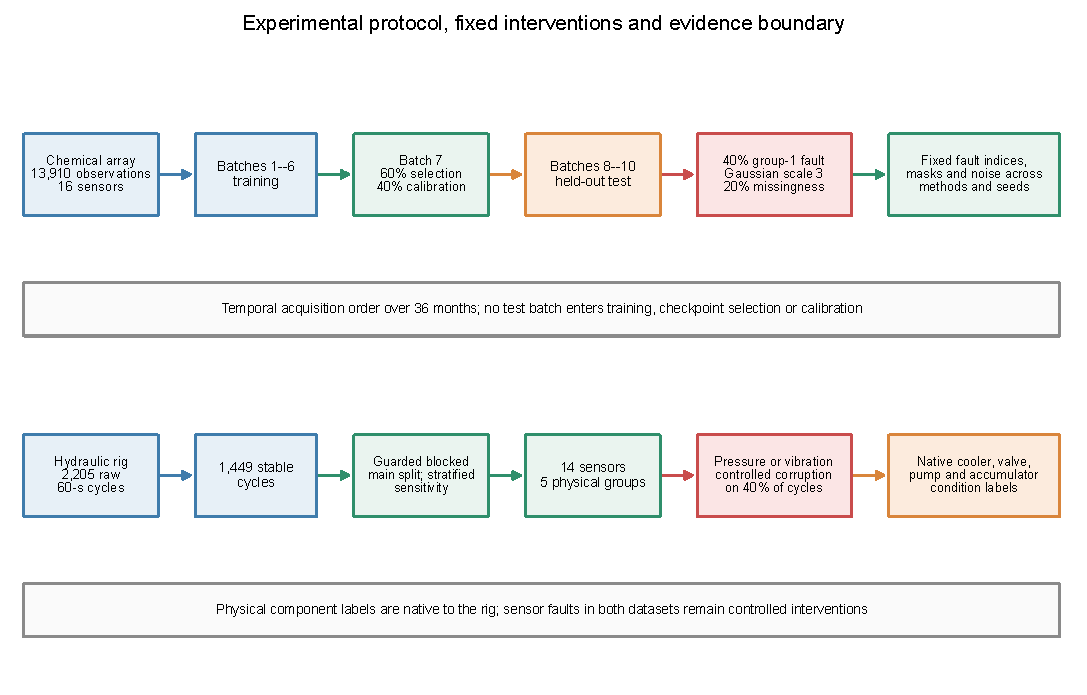
\includegraphics[width=\textwidth]{figure2_experimental_protocol.pdf}
\caption{\textbf{Integrated experimental protocol and controlled fault design.} The upper lane follows the chemical-array acquisition order from batches 1--6 training through Batch~7 checkpoint selection/calibration to held-out batches 8--10; fault indices, masks and intervention values are fixed across methods and seeds. The lower lane follows the independent hydraulic rig from stable 60-s cycles to the guarded within-condition blocked main analysis; the earlier stratified split is retained only as a sensitivity analysis. Component-condition labels are native to the rig, whereas chemical, pressure and vibration sensor corruptions remain controlled interventions.}
\label{fig:protocol}
\end{figure}
\FloatBarrier

\section{Results}

\subsection{Primary two-pass routing controlled hard-decision risk}

The strict subset contains 1,436 observations per mechanism on which the assigned intervention reached an available group. Across the 40 mechanism--seed cells, PDRF achieved mean accuracy 0.4869 and macro-AUROC 0.8115. Unconditional RO-PDRF-Lite increased these values to 0.5002 and 0.8175. Lite-CF had a 52.2\% recovery endpoint selection rate, prevented 94.7\% of recovery-induced negative transfers and retained 9.7\% of available corrections. Its accuracy and macro-AUROC were 0.4885 and 0.8151 (Table~\ref{tab:lite-main}). Thus the router controlled harmful hard-decision changes but preserved little of the unconditional endpoint's accuracy gain.

\begin{table}[ht]
\centering
\caption{\textbf{Strict-subset endpoint and routed-output quality.} Accuracy and macro-AUROC are means $\pm$ standard deviations across 10 fitted model pairs after averaging the four fixed mechanisms within each pair; remaining columns are corresponding means. These are fitting-dispersion summaries on one fixed test set. Each selector had 89.7 informative endpoint-correctness disagreements on average. Probabilities are temperature-scaled before routing; no probability mixture or post-routing recalibration is applied.}
\label{tab:lite-main}
\resizebox{\textwidth}{!}{\begin{tabular}{lrrrrrr}
\toprule
Method & Accuracy & Macro-AUROC & Macro-AUPRC & NLL & Brier & ECE \\
\midrule
PDRF & 0.4869$\pm$0.0129 & 0.8115$\pm$0.0115 & 0.5534 & 2.8239 & 0.8286 & 0.3492 \\
RO-PDRF-Lite & 0.5002$\pm$0.0089 & 0.8175$\pm$0.0105 & 0.5643 & 2.6023 & 0.7988 & 0.3302 \\
Lite-CF & 0.4885$\pm$0.0128 & 0.8151$\pm$0.0116 & 0.5598 & 2.6775 & 0.8129 & 0.3408 \\
\bottomrule
\end{tabular}
}
\end{table}

The 52.2\% selection rate and 9.7\% retention rate have different denominators. Selection is normalized by all 1,436 strict observations, whereas retention is normalized only by $N_C$, the sparse rows on which recovery alone corrects PDRF. Selection can therefore be high because the router also chooses recovery on endpoint-class agreements and rows where both endpoints share correctness status. Table~\ref{tab:opportunity-counts} reports the absolute event counts rather than only opportunity-normalized rates.

\begin{table}[ht]
\centering
\caption{\textbf{Absolute strict-subset opportunities and routed events by mechanism.} $N_C$ and $N_H$ are correction and harm opportunities; $n_C$ and $n_H$ are retained corrections and realized harms. Counts are mean absolute events per 1,436-observation fitted pair, with ranges across 10 fitted pairs in parentheses. Select uses all observations; prevent and retain use $N_H$ and $N_C$, respectively.}
\label{tab:opportunity-counts}
\scriptsize
\resizebox{\textwidth}{!}{\begin{tabular}{lrrrrrrr}
\toprule
Mechanism & $N_C$ & $N_H$ & $n_C$ & $n_H$ & Select (\%) & Prevent (\%) & Retain (\%) \\
\midrule
Gaussian & 45.9 (36--70) & 18.9 (13--32) & 6.2 (0--16) & 1.5 (0--4) & 51.9 & 91.2 & 13.5 \\
Offset & 33.6 (10--49) & 16.9 (3--37) & 2.7 (0--9) & 1.9 (0--15) & 54.1 & 93.6 & 8.1 \\
Drift & 24.7 (5--43) & 13.6 (4--29) & 1.9 (0--7) & 0.7 (0--6) & 53.9 & 97.3 & 11.1 \\
Stuck-at & 38.7 (16--86) & 17.6 (2--36) & 3.1 (0--15) & 0.7 (0--4) & 48.7 & 96.6 & 6.1 \\
\bottomrule
\end{tabular}
}
\end{table}

The routed probability vector improved on PDRF for NLL, Brier score, ECE and macro-AUPRC, but remained below unconditional RO-PDRF-Lite for every strict-set probability metric. On the complete 40\%-prevalence stream, Lite-CF/PDRF/RO-PDRF-Lite macro-AUROC values were 0.8441/0.8426/0.8451, and NLL values were 2.1386/2.2131/2.1135. On the no-imposed-fault stream, their macro-AUROCs were 0.8629/0.8631/0.8623 and NLL values were 1.8636/1.9002/1.8626. Lite-CF prevented 94.2\% of no-fault negative transfers but retained only 1.7\% of no-fault corrections, giving $-5.3$ net correct decisions per 10,000. A low residual-harm rate---the observation-level form of a harmful switch---therefore does not imply that the routed probability vector is uniformly better.

Mechanism-fixed paired intervals replace the four-cluster bootstrap (Table~\ref{tab:lite-mechanisms}). On the present fixed test set, Gaussian accuracy, AUROC and equal-cost utility differences were positive across fitted model pairs. Stuck-at AUROC was also positive, whereas its accuracy and utility intervals crossed zero. Offset and drift intervals crossed zero for most hard-decision quantities. Gaussian AUROC differences were positive within batches 8, 9 and 10 ($+0.0062$, $+0.0077$ and $+0.0061$). These intervals quantify fitting variation on fixed observations, not a population of devices or fault mechanisms.

\begin{table}[ht]
\centering
\caption{\textbf{Mechanism-fixed paired differences for the hard-decision objective.} Values are Lite-CF minus PDRF. Brackets are paired 95\% Student-$t$ intervals across 10 fitted model pairs while holding mechanism and test observations fixed. Equal-cost utility uses $V_C=C_H=1$ and $\lambda=0$. These are conditional fitting-stability summaries, not population intervals.}
\label{tab:lite-mechanisms}
\resizebox{\textwidth}{!}{\begin{tabular}{lccc}
\toprule
Fixed mechanism & $\Delta$ accuracy & $\Delta$ macro-AUROC & Equal-cost $U/10^4$ \\
\midrule
Gaussian & $+0.0033$ $[+0.0005,+0.0061]$ & $+0.0064$ $[+0.0034,+0.0093]$ & $+32.73$ $[+4.94,+60.52]$ \\
Offset & $+0.0006$ $[-0.0012,+0.0024]$ & $+0.0028$ $[0.0000,+0.0057]$ & $+5.57$ $[-12.44,+23.58]$ \\
Drift & $+0.0008$ $[-0.0006,+0.0022]$ & $+0.0018$ $[-0.0002,+0.0037]$ & $+8.36$ $[-5.69,+22.41]$ \\
Stuck-at & $+0.0017$ $[-0.0004,+0.0037]$ & $+0.0034$ $[+0.0005,+0.0063]$ & $+16.71$ $[-3.92,+37.35]$ \\
\bottomrule
\end{tabular}
}
\end{table}

The formal scale 3 intervention is a severe stress test, so we repeated the frozen test protocol at scale 1 without refitting endpoints, temperatures, selector coefficients or threshold. Lite-CF then reached 0.8357 macro-AUROC versus 0.8344 for PDRF, prevented 96.0\% of negative transfers while retaining 5.3\% of corrections and produced equal-cost utility $+4.00$ per 10,000 strict observations (Table~\ref{tab:severity-comparison}). Milder corruption improved absolute endpoint performance but left fewer useful recovery opportunities, so safety prevention did not imply greater practical benefit.

\begin{table}[ht]
\centering
\caption{\textbf{Mild and formal controlled-corruption severity.} Values are equal-weight means over four fixed mechanisms and 10 fitted model pairs on the strict subset. The scale 1 audit reuses the scale 3-calibrated selector without refitting or retuning. $U/10^4$ uses equal correction and harm values with no pass penalty.}
\label{tab:severity-comparison}
\resizebox{0.95\textwidth}{!}{\begin{tabular}{rrrrrrrr}
\toprule
Scale & PDRF acc. & Lite-CF acc. & PDRF AUROC & Lite-CF AUROC & Prevent (\%) & Retain (\%) & $U/10^4$ \\
\midrule
1 & 0.5301 & 0.5305 & 0.8344 & 0.8357 & 96.0 & 5.3 & +4.00 \\
3 & 0.4869 & 0.4885 & 0.8115 & 0.8151 & 94.7 & 9.7 & +15.84 \\
\bottomrule
\end{tabular}
}
\end{table}

At equal correction value and harm cost and without a pass penalty, Lite-CF retained 24.20 corrections and realized 8.36 harms per 10,000 strict observations, yielding net utility $+15.84$. The net values at harm-to-correction ratios 2, 5 and 10 were $+7.49$, $-17.58$ and $-59.37$. The approximate 2.9 break-even ratio is descriptive only for this endpoint pair, event definition and fixed test distribution. Complete-stream utility was negative at 0\% and 10\% controlled-fault prevalence and positive at 40\% and 70\% under equal event values (Table~\ref{tab:utility-sensitivity}). Deployment may use Lite-CF only after fixing the expected fault prevalence, correction value $V_C$, harm cost $C_H$ and compute penalty $\lambda$; energy was not measured.

\begin{table}[ht]
\centering
\caption{\textbf{Fault-prevalence and pass-cost sensitivity.} Values are means across the complete deployment streams at equal correction value and harm cost ($V_C=C_H=1$). $\lambda$ is the cost of one extra forward pass in correction-equivalents per 10,000 observations. These values are descriptive for the present endpoints and controlled test distribution.}
\label{tab:utility-sensitivity}
\resizebox{0.94\textwidth}{!}{\begin{tabular}{lrrrrr}
\toprule
Fault prevalence & Corrections/10,000 & Harms/10,000 & $U(\lambda=0)$ & $U(\lambda=0.5)$ & $U(\lambda=2)$ \\
\midrule
0\% & 1.37 & 6.65 & -5.27 & -5.77 & -7.27 \\
10\% & 3.27 & 6.93 & -3.67 & -4.17 & -5.67 \\
40\% & 8.88 & 7.33 & 1.55 & 1.05 & -0.45 \\
70\% & 15.98 & 8.36 & 7.62 & 7.12 & 5.62 \\
\bottomrule
\end{tabular}
}
\end{table}

\subsection{Sparse calibration limited selector stability}

The formal Lite-CF calibration sets contained a mean of 1,861 rows, but only 89.7 were correctness disagreements: 36.1 favoured PDRF and 53.6 favoured RO-PDRF-Lite. Frozen thresholds averaged 0.710 and ranged from 0.55 to 0.90. Across 10 repeated grouped fits per endpoint pair, mean out-of-fold AUROC was 0.720 (standard deviation 0.138; range 0.327--0.954), and thresholds ranged from 0.525 to 0.90. Applying the prospective support gate retrospectively, only 5/10 endpoint pairs passed. A descriptive gate-enforced policy therefore used recovery for 31.1\% of observations, prevented 96.2\% of negative transfers, retained 6.6\% of corrections and yielded 0.8132 macro-AUROC. The gate was added after review and does not replace the frozen headline estimand; it demonstrates how unsupported fits would revert to PDRF.

Coefficient signs were most stable for Lite confidence (94\%), base confidence (89\%) and confidence change (83\%). Dominant-sign fractions for the entropy terms were 61--67\%. Strong shrinkage traded away conditional discrimination: mean out-of-fold AUROC increased from 0.690 at $C=0.01$ to 0.717 at $C=0.05$, 0.800 at $C=1$ and 0.811 at $C=5$. The prespecified $C=0.05$ is therefore a conservative estimation choice, not the value that maximizes calibration preference AUROC.

Calibration-size sensitivity showed the same boundary. Using 25\%, 50\%, 75\% and 100\% of calibration groups produced pooled mean prevention of 88.7\%, 91.6\%, 92.4\% and 93.9\%, respectively. Retention changed from 12.1\% to 10.0\%, while macro-AUROC remained near 0.81. These are repeated-subsampling summaries and differ from the equal-weight 40-cell headline estimand.

The all-row three-outcome model and shallow tree did not dominate Lite-CF. Legacy Full-endpoint transport, staged-cascade, scalar-rule and correctness-opportunity comparisons likewise exposed unresolved trade-offs among safety, recovery, ranking and compute. Their complete estimands and tables are moved to the Supplementary Information so that the primary chain remains the PDRF--RO-PDRF-Lite--Lite-CF comparison.

\begin{figure}[p]
\centering
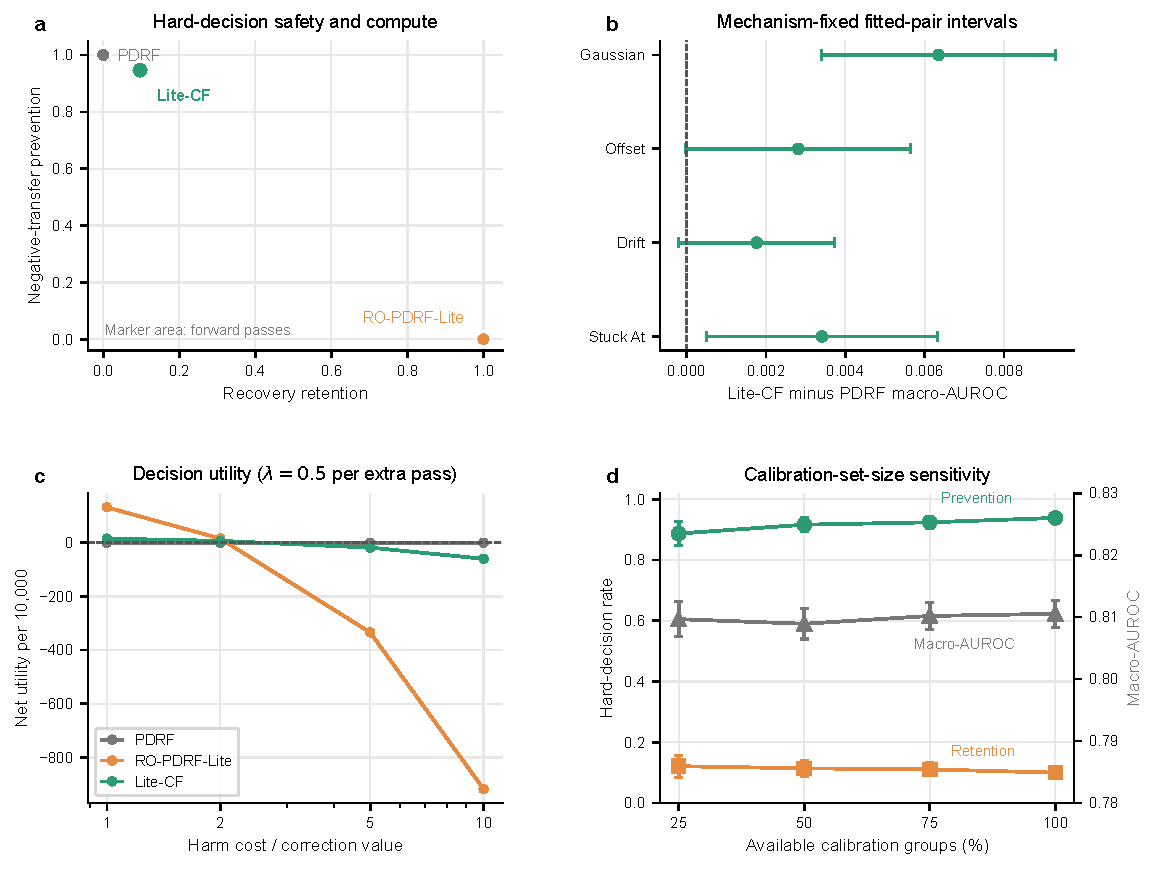
\includegraphics[width=\textwidth]{figure_cee_q1_tradeoff.pdf}
\caption{\textbf{Primary safety, mechanism and calibration evidence.} \textbf{a}, negative-transfer prevention versus recovery retention for PDRF, unconditional RO-PDRF-Lite and Lite-CF on the strict subset; marker area scales with mean forward passes. \textbf{b}, Lite-CF minus PDRF macro-AUROC with each mechanism held fixed; bars are paired 95\% Student-$t$ intervals across 10 fitted model pairs on the present fixed test set. \textbf{c}, net utility per 10,000 strict observations with $\lambda=0.5$ correction-equivalents per 10,000 for each extra pass; the inset enlarges the PDRF--Lite-CF range hidden by unconditional recovery at high harm cost. \textbf{d}, repeated calibration-group subsampling; bars show 95\% intervals over seed--repeat summaries.}
\label{fig:q1-tradeoff}
\end{figure}

\begin{figure}[p]
\centering
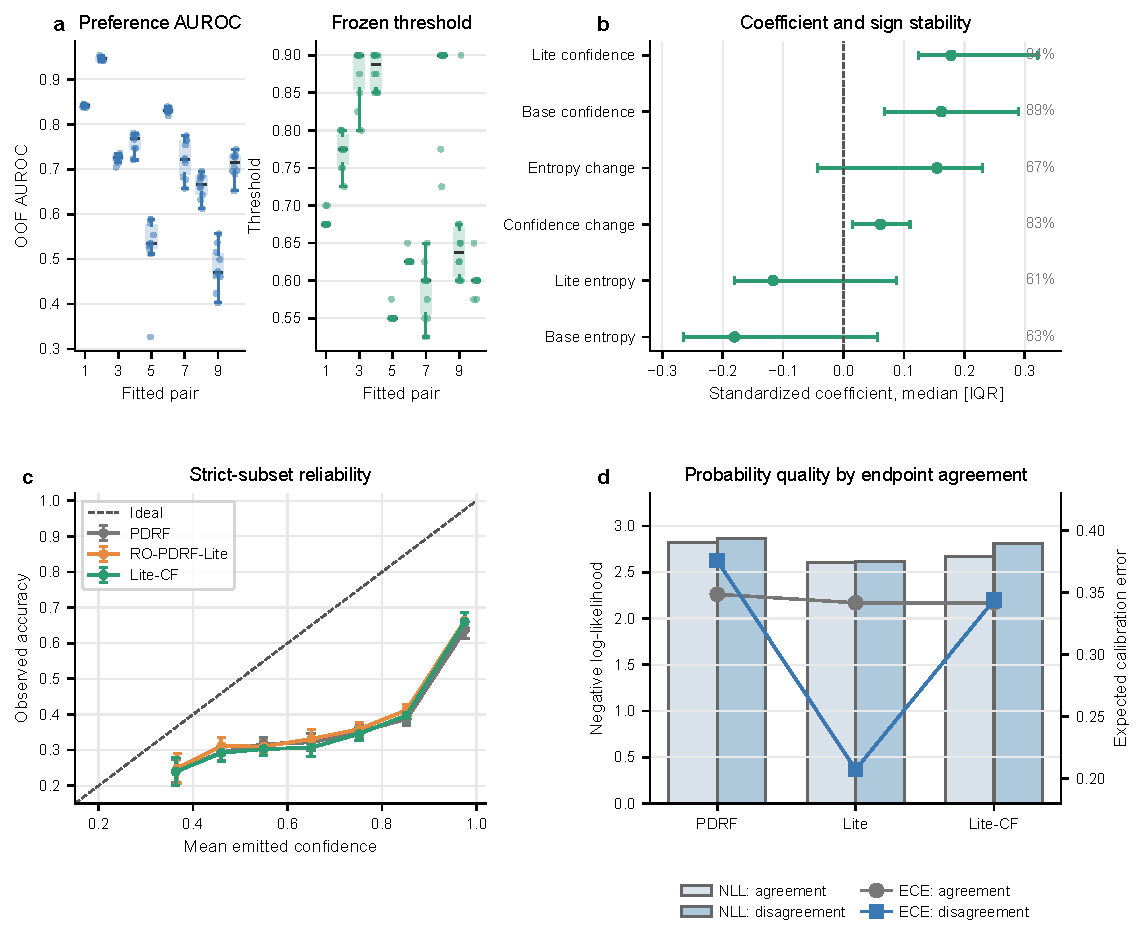
\includegraphics[width=\textwidth]{figure_cee_q1_stability_calibration.pdf}
\caption{\textbf{Selector stability and final probability quality.} \textbf{a}, seed-wise out-of-fold preference AUROC and threshold distributions across 100 repeated grouped fits. \textbf{b}, median standardized Lite-CF coefficient with interquartile range; percentages are dominant-sign frequencies. \textbf{c}, reliability curves lie predominantly below the identity line, showing substantial overconfidence for all three outputs. \textbf{d}, negative log-likelihood and 15-bin expected calibration error after separating endpoint-class agreement from disagreement. Lite-CF emits one temperature-scaled endpoint vector, not a mixture; no post-routing recalibration is fitted.}
\label{fig:q1-stability}
\end{figure}
\FloatBarrier

\subsection{Hydraulic single-rig sensitivity boundary}

The guarded hydraulic analysis used four native component-condition tasks and controlled pressure- and vibration-group faults (Table~\ref{tab:major3-hydraulic}). RO-PDRF-Full exceeded recovery-objective-matched RO-CAGF in six of eight task--fault conditions. The mean difference was $+0.015$, but the task--fault--seed hierarchical interval ($-0.006$ to $+0.036$) included zero. Performance ranged from near ceiling for cooler (RO-PDRF-Full macro-AUROC 0.996) to near chance for pump and accumulator (0.528 and 0.487), limiting architecture interpretation on the latter tasks.

The earlier random-stratified split yielded a larger mean difference ($+0.044$), indicating optimistic adjacent-cycle allocation. Guard bands reduced direct adjacency but did not create independent devices. No-interpolation and random-split results are therefore supplementary sensitivity evidence; the main result supports single-rig platform-internal robustness, not a general architecture ranking.

\begin{table}[ht]
\centering
\caption{\textbf{Hydraulic single-rig sensitivity analysis.} Guarded-block affected-subset macro-AUROC values are means $\pm$ standard deviations across five matched seeds. The eight task--fault rows are conditions from one rig, not independent devices; the earlier random-stratified results are supplementary sensitivity evidence.}
\label{tab:major3-hydraulic}
\resizebox{0.92\textwidth}{!}{\begin{tabular}{llrrr}
\toprule
Task & Fault & RO-CAGF & RO-PDRF-Full & Difference \\
\midrule
Cooler & Pressure & 0.942 $\pm$ 0.023 & 0.992 $\pm$ 0.004 & +0.050 \\
Cooler & Vibration & 0.947 $\pm$ 0.029 & 1.000 $\pm$ 0.000 & +0.053 \\
Valve & Pressure & 0.730 $\pm$ 0.026 & 0.762 $\pm$ 0.023 & +0.032 \\
Valve & Vibration & 0.739 $\pm$ 0.029 & 0.749 $\pm$ 0.032 & +0.010 \\
Pump & Pressure & 0.569 $\pm$ 0.035 & 0.536 $\pm$ 0.018 & -0.033 \\
Pump & Vibration & 0.533 $\pm$ 0.061 & 0.521 $\pm$ 0.022 & -0.012 \\
Accumulator & Pressure & 0.478 $\pm$ 0.022 & 0.491 $\pm$ 0.023 & +0.013 \\
Accumulator & Vibration & 0.474 $\pm$ 0.047 & 0.483 $\pm$ 0.044 & +0.009 \\
\bottomrule
\end{tabular}}
\end{table}

\subsection{AHU direct-diagnosis boundary}

The chronological air-handling-unit tests contained 37,831 untouched future-time records, including 2,069 expert-annotated temperature-sensor faults. Because the target is the fault itself and no independent downstream state is available, this experiment cannot test whether suppressing that sensor recovers another prediction. Early fusion exceeded bounded recovery in all 15 building--seed pairs (mean AUROC difference $-0.0341$ for bounded recovery, $P<0.001$), and leave-one-building-out bounded recovery collapsed to $0.298\pm0.005$ in the hospital. The operational data therefore establish a direct-diagnosis and transfer boundary, not downstream recovery validation; complete subtype, shift, adaptation and risk analyses remain in the Supplementary Information.

\subsection{Routed probability quality depended on endpoint agreement}

Final routed probabilities were evaluated directly rather than inferred from the residual-harm rate. Reliability curves lay predominantly below the identity line, indicating substantial overconfidence for all methods. On strict endpoint-class agreements, Lite-CF NLL/ECE were 2.667/0.342, between PDRF (2.821/0.349) and RO-PDRF-Lite (2.601/0.342). On disagreements, Lite-CF NLL/ECE were 2.813/0.344; unconditional Lite was better at 2.616/0.207, whereas PDRF was worse at 2.869/0.376. The software can expose the selected endpoint identity and conditional preference score with each probability vector. Downstream controllers should therefore treat confidence as endpoint-specific, not as one globally calibrated routed probability (Fig.~\ref{fig:q1-stability}c,d). Post-routing recalibration remains future work.
\FloatBarrier

\subsection{Lite-CF reduced, but did not remove, deployment cost}

PDRF and RO-PDRF-Lite each require one forward pass, 19,740 parameters and 38,528 counted linear-layer FLOPs per observation. Lite-CF requires two passes, 39,487 parameters and 77,056 endpoint FLOPs. With 12 intra-op threads, mean seed-level median batch-one latencies were $0.602\pm0.263$~ms for PDRF, $0.589\pm0.258$~ms for RO-PDRF-Lite and $2.471\pm0.865$~ms for Lite-CF; complete-batch latencies were $4.12\pm0.73$, $3.65\pm0.66$ and $10.21\pm2.09$~ms. At one intra-op thread, the corresponding batch-one values were $0.273\pm0.090$, $0.252\pm0.068$ and $1.553\pm0.447$~ms, and complete-batch values were $9.35\pm1.77$, $5.17\pm0.58$ and $11.60\pm0.81$~ms. All measurements used the same Intel Core i5-13500H, PyTorch 2.12.1+cpu, three warm-ups and seven timed calls, excluding loading. They do not establish embedded latency, energy efficiency or real-time readiness.

\section{Discussion}

The strict estimand and frozen-run discipline narrow the central interpretation. Clean-to-faulted distillation produced a useful recovery endpoint, but unconditional gains varied by mechanism. The contribution is therefore a risk-control protocol, not a universal fusion architecture. It distinguishes fault assignment from an intervention that reaches an available group, measures correction and error transfer, and freezes routing before test evaluation.

Cross-fitting addresses threshold leakage, not sparse-event estimation. Only 89.7 correctness disagreements informed each selector on average, and repeated fits exposed unstable discrimination, thresholds and entropy coefficients. The prospective event, AUROC and threshold-stability gate accepted only 5/10 endpoint pairs. Unsupported sites must use PDRF while collecting new calibration evidence. Neither coefficients nor thresholds should transfer between fitted deployments.

The safety--recovery trade-off remains substantial. Lite-CF prevented 94.7\% of negative transfers while retaining only 9.7\% of corrections. Its 52.2\% recovery endpoint selection rate is larger because selection uses all observations, whereas retention uses rare correction opportunities. At scale 1, prevention rose to 96.0\% but retention fell to 5.3\% and equal-cost utility to $+4.00$ per 10,000. Complete-stream utility was negative at 0\% and 10\% fault prevalence, and the strict preference reversed above the descriptive 2.9 harm-to-correction ratio. Deployment therefore requires externally fixed prevalence, event values and compute cost.

The two-pass design avoids leave-one-group-out inference but stores and evaluates two models. Fixed 1-thread and 12-thread measurements confirmed additional batch-one latency. Workstation values do not establish embedded latency, memory-bandwidth adequacy, energy use or real-time readiness, so the utility analysis retains explicit pass and FLOP proxies.

Mechanism-fixed and batch-fixed intervals replace the four-mechanism population bootstrap. Gaussian differences were positive across fitted pairs on the present fixed test set; several offset, drift and stuck-at hard-decision intervals crossed zero. All intervals reuse one instrument and the same observations. They quantify fitting variation, not sampling from devices or natural faults. Scale 3 is also a severe standardized stress test, while scale 1 shows that milder corruption does not automatically increase routing utility.

Transfer tests define boundaries rather than confirm field recovery. The hydraulic result is single-rig sensitivity, and its guarded architecture interval crosses zero. The AHU target is the sensor fault itself, so diagnosis may reward signatures that recovery suppresses. A prospective study must include multiple independently operated devices, maintenance-adjudicated sensor failures and downstream targets that do not encode those failures. Endpoint fitting and site-specific calibration must precede outcome analysis, with the support gate, PDRF fallback and utility values frozen in advance.

Further boundaries remain. Routed probabilities are overconfident and endpoint-specific; no tested output dominates safety, ranking and calibration. Response saturation prevents device-health interpretation, and erroneous clean teachers or quality metadata can transfer errors. Evidence remains limited to controlled feature corruption, one chemical instrument, one hydraulic rig and expert/rule-based AHU labels. Multi-device prospective evaluation is required before field-recovery claims.

\section{Conclusion}

Cross-fitted selective recovery converted a useful but fallible recovery endpoint into an explicit deployment trade-off. On the strict controlled-corruption estimand, Lite-CF prevented 94.7\% of negative transfers while retaining 9.7\% of corrections; it is a conservative safety layer, not a generally improved classifier. Utility was negative at low complete-stream fault prevalence and remained application-specific. Only 5/10 fitted endpoint pairs met the prospective event, discrimination and threshold-stability gate, requiring PDRF fallback for the remainder. Mechanism-fixed and mild-severity audits further showed that benefits were not uniform. Routed probabilities remained endpoint-specific and overconfident. The contribution is a reproducible hard-decision risk-control protocol for controlled available-group corruption, not evidence for calibrated device health, natural-failure recovery or device-independent field performance.

\section*{Data and code availability}

The Gas Sensor Array Drift Dataset (DOI: \url{https://doi.org/10.24432/C5RP6W}) and Condition Monitoring of Hydraulic Systems dataset (DOI: \url{https://doi.org/10.24432/C5CW21}) are available from the UCI Machine Learning Repository under CC BY 4.0. The operational AHU data are available from Figshare under CC BY 4.0 (DOI: \url{https://doi.org/10.6084/m9.figshare.27147678.v3}). Code, fixed seeds, environment information, source data for CEE-CF10-R2-LITE and figure/table scripts are publicly available in the \texttt{cee\_revision} directory at \url{https://github.com/Corey9999/recovery-supervision-calibrated-fallback}. The frozen Strict-88 computational snapshot is commit \texttt{12a74760d350e934297a9e4be9e44d63a44a0655}; the versioned submission release is \texttt{v1.3.0-strict88}. Exact dependencies are recorded in \texttt{requirements-lock.txt} and \texttt{environment.yml}, and the script-to-result manifest is Supplementary Table~S1. A permanent software DOI has not been assigned.

\section*{Ethics statement}

The study used public engineering datasets and controlled computer-generated sensor corruptions. It involved no human participants, personal data, animals or biological specimens; institutional ethics review was not applicable.

\section*{Author contributions}

Riyang Luo: Conceptualization, Methodology, Software, Validation, Formal analysis, Investigation, Data curation, Visualization, Writing--original draft, Writing--review and editing, and Project administration.

\section*{Acknowledgements and funding}

The author received no specific funding for this work and has no acknowledgements to declare.

\section*{Declaration of interests}

The author declares that there are no known competing financial interests or personal relationships that could have appeared to influence the work reported in this paper.

\bibliographystyle{unsrtnat}
\bibliography{references}
\end{document}
